\section{Peer-2-Peer}{P2P}
Esta aula é expositiva, mostrando como as DHT evoluiram do Chord,  essencialmente de uso acadêmico, para aplicações industriais na forma de bancos de dados como o Cassandra e o DynamoDB.

\subsection[Intro]{Introdução}

\begin{frame}{Sistemas Peer-2-Peer}
\begin{itemize}
	\item Características
	\begin{itemize}
	\item Arquitetura decentralizada
	\item Não há distinção de papéis entre nós, ou papéis tem igual relevância.
	\item Não há servidores e clientes, mas iguais (pares) na computação.
	\item Nós entram e saem frequentemente.
	\item Redes sobrepostas (\emph{overlay}).
	\end{itemize}
	\item Objetivos
	\begin{itemize}
	\item Alto desempenho
	\item Escalabilidade geográfica global
	\item Auto-administração
	\item Tolerância a falhas
	\end{itemize}
\end{itemize}
\end{frame}

\subsection[DHT]{Distributed Hash Tables}

As tabelas hash tem uma interface muito simples de armazenamento de dados, sendo adequadas a vários cenários.

\begin{frame}[fragile]{Mapa/Dicionário/Array Associativo/Hash Table}
Estrutura de dados que \emph{mapeia} uma chave para um valor.
\begin{itemize}
	\item $f(K): V \cup$ \{null\}
	\item $K$: Universo de chaves
	\item $V$: Universo de valores
	\item isto é, $f(k) = v, k\in K, v \in V$ ou $v =$ null.

\pause
	
	\item API Simples
	\begin{itemize}
		\item v' = put(k,v) //Retorna valor já existente
		\item v' = update(k,v) //Retorna valor já existente
		\item v' = get(k) //Retorna valor já existente
		\item v' = del(k) //Retorna valor já existente
	\end{itemize}
	\item $v$ é um blob
	\item Tempo de execução (mais ou menos) constante
\end{itemize}
\end{frame}

\begin{frame}[fragile,allowframebreaks]{Distributed Hash Tables}
Como distribuir um HT de forma que
\begin{itemize}
\item mantenha API e funcionalidade
\item agregue as capacidades de diversos hosts?
\end{itemize}

Desafios incluem
\begin{itemize}
\item O que usar como chave?
\item Como dividir carga (uniformemente) entre hosts?
\item Como rotear requisições para o host correto?
\end{itemize}
\end{frame}


\begin{frame}{Identificação}
\begin{itemize}
	\item Identificação única por objeto
	\item Identificador atribuído pela aplicação
	\item Exemplo, CPF da pessoa
\end{itemize}
\end{frame}

\begin{frame}{Divisão de carga}
\begin{itemize}
	\item Cada nó é responsável por uma faixa de valores
	\item 000.000.000-00 -- 111.111.111-00 -- Host1
	\item 111.111.111-01 -- 222.222.222-00 -- Host2
	\item 222.222.222-01 -- 333.333.333-00 -- Host3
	\item ...
\end{itemize}
\end{frame}

\begin{frame}{Divisão de carga}
\begin{itemize}
	\item Nomes
	\item A -- C -- Host1
	\item CA -- E -- Host2
	\item EA -- G -- Host3
	\item ...
\end{itemize}
\end{frame}

\begin{frame}{Divisão de carga}
A distribuição não é boa. 

Depende da distribuição dos dados.
\end{frame}



\begin{frame}{Identificação}
\begin{itemize}
	\item Seja $i$ o identificador do objeto, dado pela aplicação (e.g., CPF, nome)
	\item Seja $h$ uma função criptográfica
	\item $k = h(i)$ tem distribuição uniforme
	\item Por exemplo, MD5 tem $2^{160}$ possíveis valores
	\item Distribua os valores entre os hosts
\end{itemize}
\end{frame}

\begin{frame}{Roteamento}
\begin{itemize}
	\item Cada nó é responsável por um \emph{bucket}
	\item Chave $k$ vai para bucket é $k \% b$, onde $b$ é o número de buckets
	\item Como associar um bucket a um nó?
	\item Redes sobrepostas
\end{itemize}
\end{frame}

\begin{frame}{Redes Sobrepostas}
\begin{itemize}
	\item Uma rede lógica sobre uma rede física
	\item Conexões consideradas canais de comunicação
	\item Roteamento no nível da aplicação
	\item Estruturadas e não-estruturadas	
\end{itemize}

\pause
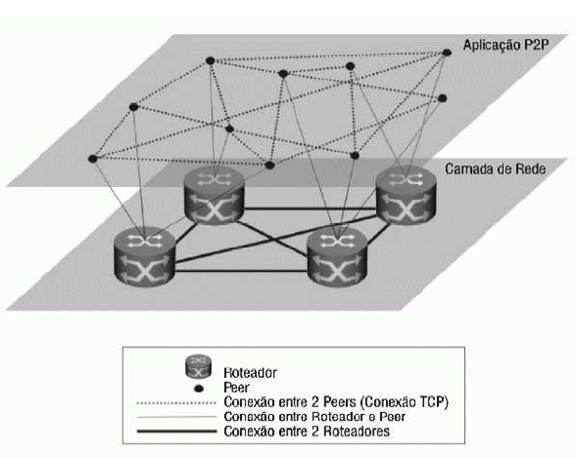
\includegraphics[width=.5\textwidth]{images/overlay}

\href{https://content.iospress.com/media/jhs/2017/23-1/jhs-23-1-jhs558/jhs-23-jhs558-g002.jpg?width=755}{Fonte}

%\includegraphics[width=.5\textwidth]{images/Network_Overlay}
%Fonte: \href{https://commons.wikimedia.org/w/index.php?curid=10086213}{Ludovic.ferre}
\end{frame}


\subsection{Chord}

\begin{frame}{Chord}
\begin{beamerboxesrounded}{Chord e derivados}
	\begin{itemize}
		\item CSAIL (MIT) -- 2001
		\item Anel lógico
		\item Identificadores de nós: m-bits
		\item Identificadores de dados: m-bits
		\item Dado associado a um nó/identificador
		\item Dado com chave $k$ é responsabilidade do nó com menor identificador $i \geq k$, aka sucessor de $k$ ($i = suc(k)$)
	\end{itemize}
\end{beamerboxesrounded}

\pause
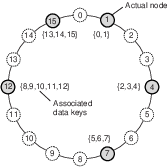
\includegraphics[width=.45\textwidth]{images/02-07}	
\end{frame}

\begin{frame}{Chord }
\begin{beamerboxesrounded}{Chord e derivados}
Roteamento?
\end{beamerboxesrounded}

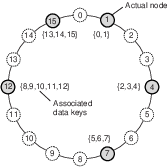
\includegraphics[width=.45\textwidth]{images/02-07}	
\end{frame}


\begin{frame}{Chord}
\begin{beamerboxesrounded}{Roteamento eficiente}
	\begin{itemize}
		\item Sucessores
		\item Finger-table
	\end{itemize}
\end{beamerboxesrounded}

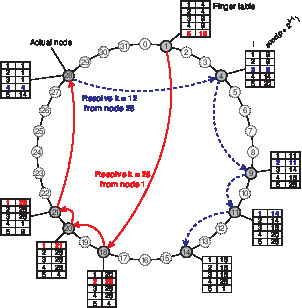
\includegraphics[width=.45\textwidth]{images/05-04}	
\end{frame}

\begin{frame}{Chord}
\begin{itemize}
	\item $FT_p[i] = suc(p+2^{i-1})$\\
	$FT_p[i]$ aponta para primeiro nó que sucede $p$ por pelo menos $ 2^{i-1}$
	\item Para achar nó responsável por $k$, $p$ encaminha requisição para nó na entrada $j$ tal que $FT_p[j] \leq k < FT_p[j + 1]$
\end{itemize}

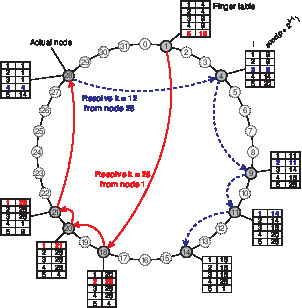
\includegraphics[width=.45\textwidth]{images/05-04}	
\end{frame}

\begin{frame}{Chord}
\begin{itemize}
	\item Menor/Maior?
	\item 21 procurando 31?
\end{itemize}

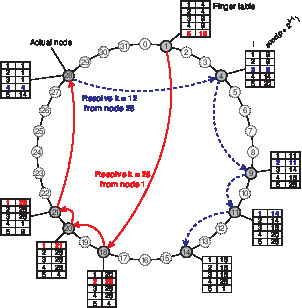
\includegraphics[width=.45\textwidth]{images/05-04}	
\end{frame}

\begin{frame}{Churn}
\begin{itemize}
	\item Entrada e saída de nós
	\begin{itemize}
		\item Se sou o nó X e quero entrar na rede
		\item Quem é o sucessor S de X?
		\item Quem é o antecessor A do sucessor de X?
		\item Reconfigure S e A
	\end{itemize}
\end{itemize}
\end{frame}

Reorganização dos nós exige movimentação de dados. Como minimizar o impacto da reorganização? Ou pelo menos balanceá-la?

\begin{frame}{Churn}
\begin{itemize}
	\item Movimentação de dados
	\begin{itemize}
		\item Se sou novo na rede, parte dos ``meus'' dados estão com meu sucessor.
		\item Copie o dados
		\item Como satisfazer requisições durante o processo?
	\end{itemize}
	\pause
	\item Sucessor fica sobrecarregado provendo dados
	\item Nós virtuais
	\begin{itemize}
		\item Cada nó físico assume vários identificadores
		\item Movimentação é distribuída entre nós
	\end{itemize}
\end{itemize}
\end{frame}

\begin{frame}
Consistent hashing
\end{frame}



Pela replicação dos dados, consegue-se minimizar o impacto de falhas no sistema. 
\begin{frame}{Falhas}
\begin{itemize}
	\item Além do sucessor, conhecer sucessor do sucessor
	\item Em caso de suspeita de falha, reorganize ponteiros
	\item Perda de dados
	\pause
	\item Replicação para vizinhos
	\item Degradação graciosa
\end{itemize}
\end{frame}

\begin{frame}{Fator de replicação: $r$}
\begin{itemize}
	\item Para cada dado, há $r$ cópias
	\item Conflito: aquele que tem o maior \emph{vector clock} vence
	\item Versões concorrentes são resolvidas com abordagem genérica: pergunte ao operador.
\end{itemize}
\end{frame}





Nestes ``bancos de dados'' distribuídos, pode-se optar por uma alta latência ou por um modelo de consistência eventual, no caso bem comportado; no caso de falhas, espera-se que a consistência seja eventualmente alcançada, mas não se pode garanti-la.
\begin{frame}{Aplicações}
\begin{itemize}
\item Replicação + assincronismo = inconsistências
\item consistência eventual 
\end{itemize}
\end{frame}

\subsection{DynamoDB}

Este modelo é adequado a algumas aplicações, como o carrinho de compras da Amazon.com
\begin{frame}{Dynamo DB -- Consistência Eventual}
\begin{itemize}
\item \emph{Shopping Cart} da Amazon.com
\item Chave: identificador do usuário
\item Valor: conteúdo do carrinho de compras
\item Modificações do carrinho criam novas versões\\  \alert{Consistência eventual}
\item O que acontece no caso de falhas? Atrasos? \\   \alert{Múltiplas versões!}
\item E no caso de o carrinho ficar errado?
\end{itemize}

\url{http://aws.amazon.com/dynamodb/}
\end{frame}

O modelo de blob do Dynamo impõe algumas restrições de uso para o desenvolvedor.

\begin{frame}{Esquema de Dados}
\begin{itemize}
\item Valor no DynamoDB é um \alert{blob}
\item Serialização e desserialização é um problema menor
\item Entradas tem um Version Vector como versão
\item Quais os dados com chave entre X e y?
\end{itemize}
\end{frame}


\subsection{Cassandra}
O Cassandra, com seu modelo híbrido chave-valor/relacional, facilita o desenvolvimento de certas aplicações.

\begin{frame}{Apache Cassandra}
\begin{itemize}
\item Híbrido entre chave-valor e relacional
\item Valores, ou linhas, são agrupados em \emph{column families} (equivalente a tabelas)
\item Column Families, juntas formam um \emph{keyspace} (equivalente a um banco de dados)
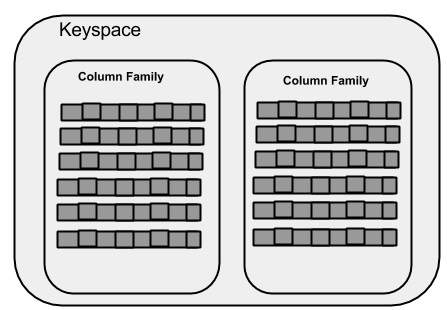
\includegraphics[width=.7\textwidth]{images/cass_keyspace}
\end{itemize}
\end{frame}


\begin{frame}{Apache Cassandra}
\begin{itemize}
\item Chave mapeia para um conjunto de colunas
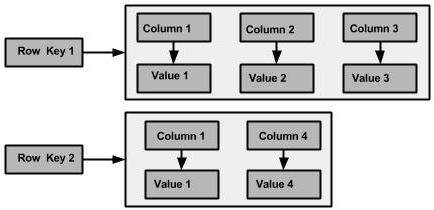
\includegraphics[width=.7\textwidth]{images/cass_column_family}

\item Cada coluna tem valor e timestamp
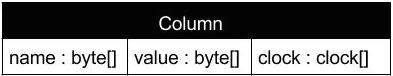
\includegraphics[width=.7\textwidth]{images/cass_column}


\item Linhas podem ser ordenadas por valores de algumas colunas (chave composta)

\item Colunas podem ser agrupadas em {\emph super-columns}\\
(Não recomendado)

%\item \emph{Range Queries} -- todas a linhas com chave em determinada faixa de valores
\end{itemize}
\end{frame}




\begin{frame}[fragile,allowframebreaks]{Apache Cassandra}
\begin{itemize}
\item Super-column families

%\begin{verbatim}
%UserList={    <- Table (Tables pertencem a um keyspace)
%     Cath:{   <- Chave
%         //Super column
%         username:{firstname:”Cath”, lastname:”Yoon”}
%         address:{ city:”Seoul”,postcode:”1234”}}
%           
%     Terry:{   //Super columns formam super column families
%         //Columns formam column families.
%         username:{firstname:”Terry”,lastname:”Cho”}
%         account:{bank:”hana”,account:”1234”}}
%}
%\end{verbatim}

\item Cassandra Query Language
\end{itemize}

\url{http://wiki.apache.org/cassandra/FrontPage}
\end{frame}


\begin{frame}{Demo}
\url{https://blog.rackspace.com/cassandra-by-example}

\url{http://wiki.apache.org/cassandra/GettingStarted}	
\end{frame}

É possível rodar o Cassandra facilmente em certas nuvens computacionais.


E há vários exemplos de aplicações desenvolvidas usando-se o cassandra.
\begin{frame}{Twissandra}
\url{https://github.com/twissandra/twissandra}
\end{frame}



\begin{frame}{Aplicação}
\url{https://github.com/datastax}

\url{https://github.com/datastax/java-driver}

\url{http://downloads.datastax.com/java-driver/cassandra-java-driver-3.0.0.tar.gz}

\url{http://www.devjavasource.com/cassandra/cassandra-crud-operation-using-java/}
\end{frame}


\begin{frame}{Para aprender mais}
\url{http://www.tutorialspoint.com/cassandra/}	
\end{frame}


\begin{frame}{Caso de uso: resolução de nomes}
\begin{itemize}
	\item \url{http://ufu.br}: IP
	\item \url{http://pop3.mail.ufu.br}: IP
	\item \url{/home/lasaro/public_html/sites/disciplinas}: INode
	\item \url{+55 34 99924 2358}: IMEI 
\end{itemize}

Como você implementaria usando uma DHT?
\pause
Chave normalizada
\end{frame}





%TODO: \subsection{CAN}



\subsection[Estrutura]{Redes Estruturadas e Não estruturadas}

\begin{frame}{Redes Sobrepostas}
\begin{block}{Estruturadas}
	\begin{itemize}
		\item Estrutura bem definida
		\item Adição de dados é lenta
		\item Adição de nós é lenta
		\item Busca por dados é rápida
	\end{itemize}
\end{block}
\begin{block}{Não Estruturadas}
	\begin{itemize}
		\item Estrutura aleatória
		\item Adição de dados é rápida
		\item Adição de nós é rápida
		\item Busca por dados lenta
	\end{itemize}
\end{block}
\end{frame}


\begin{frame}{Estruturadas}
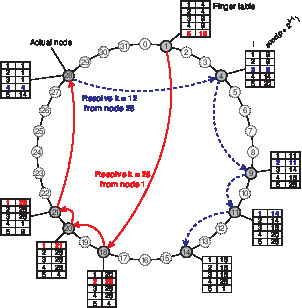
\includegraphics[width=.45\textwidth]{images/05-04}	

\begin{itemize}
	\item Inserção de nós requer atualização de informações
	\item Busca usa tabela de roteamento
\end{itemize}
\end{frame}

\begin{frame}{Estruturadas}
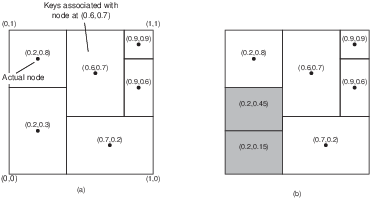
\includegraphics[width=.7\textwidth]{images/02-08}	

\begin{itemize}
	\item Cada nó é responsável por uma área
	\item A inserção/remoção de um nó causa um split/merge
\end{itemize}
\end{frame}

\begin{frame}{Não estruturada}
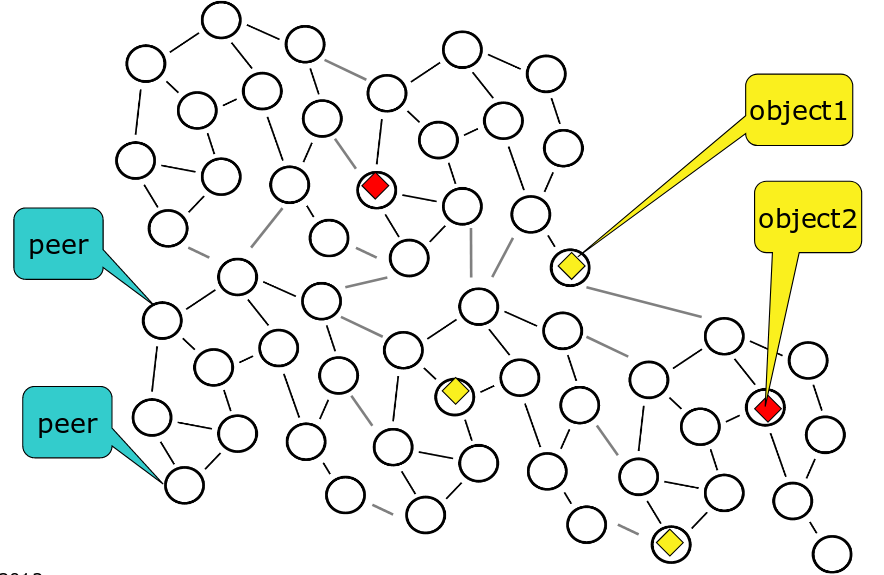
\includegraphics[width=.6\textwidth]{images/unstructured}	

\begin{itemize}
	\item Inserção afeta apenas nós contactados
	\item Busca requer varredura (p.e., inundação, random walk), ou índice
\end{itemize}


\href{http://gossple2.irisa.fr/~akermarr/LSDS-EPFL-unstructured.pdf}{Fonte}
\end{frame}


\begin{frame}{De não estruturada a estruturada}
%\includegraphics[width=.6\textwidth]{images/3d_thorus}	
%\href{https://clusterdesign.org/torus/}{Fujitsu and RIKEN, 2009}

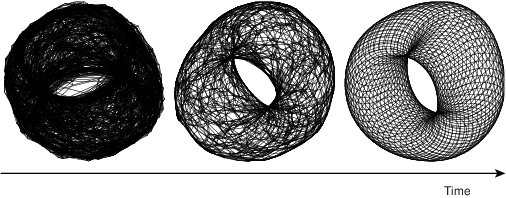
\includegraphics[width=.6\textwidth]{images/02-11}	

\pause

Seleção de links segundo critério

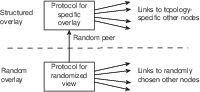
\includegraphics[width=.6\textwidth]{images/02-10}	

\pause
Seja uma grade $N \times N$. Mantenha nós mais próximos:
\begin{itemize}
	\item $a = (x,y)$, $b = (x', y')$
	\item $dx_{a,b} = min(|x - x'|, N - |x - x'|)$
	\item $dy_{a,b} = min(|y - y'|, N - |y - y'|)$
	
\end{itemize}
\end{frame}

